\section{Approach}
%Here what we propose?

%In this project, we intend to use attacks on ADS, to model faults activated in sensors and the communication channels present in an autonomous driving systems. We intend to study the effect of such fault activation (for example, corruption of reported sensor values, corruption of communication channel between sensor and the control system, unexpected activities in hardware controlling the sensor due to faults in control logic etc.) on the output of the entire ADS system.This is an unexplored area and the first step in this research involves formulating of attack models for individual sensors. These attack models will then be used to systematically inject faults in the system and then find vulnerable states in the system.

%We intend to compare the results of this systematic FI with to the existing fault injecting techniques and compare the performance and accuracy of these system by answering following questions. 

%\begin{itemize}
%\item  Does employing systematic approach to FI increase the performance in comparison to fuzz testing?

%\item Does benefit obtained in terms of performance justify the effort required for developing systematic approaches for FI?

%\end{itemize}
%The information collected using these individual attack models will then be used to find the vulnerabilities in the integrated ADS system. To detect and provide resilience against detected vulnerabilities, we will develop a model-based analysis framework, based on the dynamics of the ADS in order to test for any behavior not corresponding to system specifications.

%We propose development of a systematic method to find vulnerabilities in components of an ADS, instead of using standard ad-hoc approaches~\cite{jha18dsn}~\cite{jha18art}, which don't provide good coverage for resilience assessment. The main objective of this project will be to develop a technique that can detect all vulnerabilities in sub-components that lead to degradation of reliability of whole system. This is an unexplored area and the first question in this research will be to find out, if this method is feasible. This involves formulating of fault models for individual components of an ADS. After development of fault models, individual components will be manually tested for vulnerabilities to test the validity of these fault models. This testing will be generalized and automated later by developing a tool that systematically finds all the vulnerabilities specified by the fault model of a component. The information collected using these individual fault models will then be used to find the vulnerabilities in the integrated ADS system and improve its resilience.

%CARLA will be used as a test platform for development and testing of our approach as it provides a convenient way to instrument and modify the readings of different sensors, as well as the behavior of driver agents that controls the autonomous vehicle. 

%Current approaches that analyze resilience of ADS systems on a holistic level perform fault injections to find vulnerabilities in the system which is quite resource intensive. Details about such approaches is provided in section \ref{related_work}. Our proposed methodology will forgo such ad hoc approaches and test different components of an ADS in a systematic way by modeling its behavior and using formal methods to validate its correctness and finding any unexpected behavior that introduces vulnerabilities in the ADS system. 

% Our contribution
Our contribution is two-fold in this work. First, by an in depth understanding of autonomous vehicles, we device a fault model for the vehicle in general. We specifically focus on the sensor faults and design a fault-model specific to the sensors. Second, based on our fault model, we inject faults in order to obtain the failure rate of the system caused due to the sensor faults. We attempt fault injection in order to get maximum coverage of the system in an optimal manner.

\subsection{Fault-model for ADS}
% general categorization of the fault-model
Analyzing the system, we designed a fault model for autonomous driving systems. We categorized the fault occurrence in two ways: due to some physical damage or due to network issues. These two categories of faults cover almost all possible components of the systems which can lead to a failure of the system. 

%\\TODO- components of the LIDAR.





%why do we define the fault-model of the entire system
In Figure~\ref{fig:fault-modelgeneral} we try to give a complete fault model of autonomous vehicles. However, covering the failures caused by each component is out of scope of our current paper. Also, analyzing failure rates in general instead of component wise failure rates will not provide us with useful set of results. Hence we built a complete fault-model of the system initially. After building a comprehensive fault-model, based on our judgment, we decided to focus on one of the core set of components of ADS.

%Core Components we selected for faults in ADS
 The core component we selected were the  sensors used in ADS. However, every sensor used in ADS is very detailed oriented and performs multiple functionalities. So out of the four major sensors which we have explained in further details in Section 3, we focused on LIDAR. 
 
 \subsection{Fault-model of LIDAR}
 %A little more about LIDAR
 LIDAR is a very expensive sensor and hence finding the failure rates of the system, caused due to LIDAR can help the designers understand how to mitigate the faults such that they don't lead to failures. ADS being safety critical systems, can cause a lot of harm ( death in the worst case scenario ) in case of a failure. 
 
 \subsubsection{Hardware faults} These faults represent the soft errors that can occur in the data that is recorded by the sensors. These faults can occur in the registers of sensor units, in communication links between sensor and control unit and with in registers where these values are stored in the main ADS controller. Regardless of the location where the fault occurs, we assume that it is always activated and observed by the client when it reads the sensor data. This type of faults in real life can introduce single and multiple bit flips randomly in the sensor readings, which is modeled by our FI technique.
 
 \subsubsection{Data Faults} These faults refers to the condition in which the sensors give a readings which are not correct according to the environment. These faults can occur due to manufacturing defects in the sensors and various environmental conditions. Environmental conditions can refer to weather and other characteristics of the surroundings that are used in decision making process by the ADS (e.g. lane markings on road). For example, A LIDAR mapping its surrounded by laser can be effected by rainy weather such that the laser bouncing from the surrounding objects is effected by rainy weather thus the mapping produced by LIDAR is not representative of real environment.
 
\begin{figure}
 	\centering
 	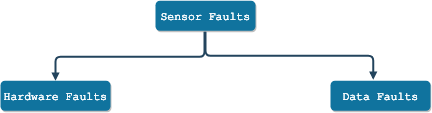
\includegraphics[width=1.0\linewidth]{Sensor-faults}
 	\caption{In the sensor faults (LIDAR), we consider hardware and data faults. }
 	\label{fig:sensor-faults}
\end{figure}

 %LIDAR fault model
 We will be providing the fault-model for ADS in our final report.
 
\section{Research Implementation}
%Abdul this is your section so check the subsections you are supposed to work on from our discussion notes.

\subsection{Fault Injection} \label{fi_m}

% Done - PICK UP FIRST SECTION FROM THE NEXT SECTION AND PUT IT HERE. 

In our study with random Fault injection we study each fault separately, so for a set of related experiments we only inject one type of fault. Only one fault is injected in each execution run and its effect on the overall operation is observed. The goal and path to navigate is constant in each trial so that outcome of each trail can be compared with output of a golden run, in which no fault was injected. 

\begin{figure}  
	\vspace{-0.5em}
	\centering
	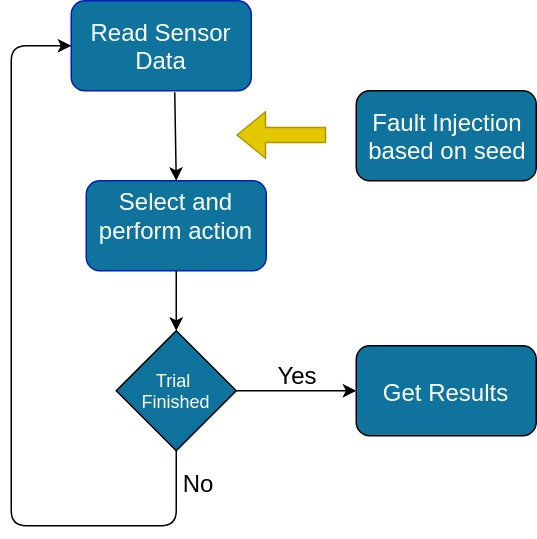
\includegraphics[scale=0.3]{FI_method}
	\vspace{-0.5em}
	\caption{Life cycle of an experiment trial on client side, Fault is injected by altering sensor readings received by client.}
	\label{fig:FI_method}
	\vspace{-1.5em}
\end{figure}

% THESE ARE THE TYPES OF FAULTS AND HOW ARE YOU INJECTING????
\textcolor{red}{We need a text block about how we represent different faults and justify it, from literature review}

As mentioned in~\ref{ri-carla} CARLA provides a client server architecture. We exploit this boundary between client and server for our fault injection experiments. Figure~\ref{fig:FI_method} provides an overview of method of fault injection used in one trial. The CARLA platform provides an ability to run multiple trails of the same experiments (same environment and goals). Each trial involves multiple steps. In each step, data is read from the sensors, this data is provided to the controller which based on some predefined algorithm and current sensor readings, gives command to the AV, after the command, it is checked if the objective of the trial is achieved or the timeout has happened. If any of these condition exists, we end the current trial and the using the measurements from the server, the metrics defined in~\ref{fi_m} are calculated for this trial and after that we move on to the next trial. 

The sensor readings are provided in form of dictionary to driving agent from the client, which can be easily accessed in the code. We insert a code block in between reading data from server and sending it to driving agent. This code block changes the reading of the sensor under study based on the fault that we are testing.

We use the following metrics to quantify the resilience of ADS which are inline with previous work in this domain~\cite{avfi}.
\setcounter{subsubsection}{0}

\medskip
\subsubsection{Success percentage} This metric represents the fraction of total trials in which the ADS was successful in achieving the specified target when faults are injected.

\smallskip

\subsubsection{Violations per trial} This metric captures the traffic violations that occur during each trial. The violations that we consider for calculating this metric are lane violation and curb violations (reasons for not considering collisions with dynamic objects are explained in \ref{ri-carla}). 

The two metrics used, provide and opportunity to study the effects of faults on the overall functioning of AV as well as the lower level deviations from normal behavior, which may not lead to outright failure but violate safety properties.

% Moved from the other section here

%\subsection{Fault Injection method} \label{method}

\section{Evaluation}
In this section we present the fault model for the sensors. We further evaluate the failure rates caused due to the faults in the sensor. We address the following research questions:
\begin{enumerate}
	
\end{enumerate}